\documentclass[12pt,letterpaper]{article}
\usepackage[spanish]{babel}
\usepackage[utf8]{inputenc}
\usepackage[right=3cm,left=3cm,top=2cm,bottom=2cm,headsep=0cm,footskip=0.5cm]{geometry}
\usepackage[dvips]{graphicx}
\usepackage{verbatim}
\usepackage{multicol}
\usepackage{fancyvrb,relsize}
\usepackage{amsthm}
\usepackage{amssymb}
\usepackage{listings}
\usepackage{wrapfig}
\usepackage{subfig}
\usepackage{placeins}
\usepackage{setspace}
\usepackage{amsmath}

\begin{document}
\begin{titlepage}
\begin{figure}[ht]

\includegraphics[scale=1]{logo_departamento.eps}
\label{DCC}
\vspace{1cm}
\end{figure}
\begin{center}
\vspace{4cm} {\Huge Tarea 3: Skip Lists y ABB Aleatorizados}

\vspace{1cm} {\Large CC4102 - Diseño y Análisis de Algoritmos}
\vspace{7.5cm}
\end{center}

\begin{tabbing}
\hspace*{7cm}\=\hspace*{3.5cm}\= \kill

\> {\large Profesor:} 	\> 	{\large Gonzalo Navarro} \\ \\
\> {\large Auxiliar:}	\> 	{\large Teresa Bracamonte} \\ \\
\> {\large Alumnos:}	\> 	{\large Cristián Carreño} \\ \\
\> {\large } 			\> 	{\large Sergio Maass} \\ \\
\> {\large Fecha:} 		\> 	{\large 18 de Diciembre de 2013}
\end{tabbing}

\end{titlepage}
%\begin{doublespace}

\tableofcontents
\newpage

\section{Introducción}
Los Skip Lists (SL) son estructuras de datos que permiten almacenar objetos en listas enlazadas ordenadas. A diferencia de las listas enlazadas convencionales, los skip lists aleatorizan el algoritmo de inserción de forma que cada vez que se inserta un nuevo elemento, se pueden generar $d$ duplicados aleatoriamente de forma que estos compongan un atajo para la lista enlazada original y reduzcan el tiempo de búsqueda. La ventaja de los skip list es que aseguran un tiempo promedio de búsqueda de $O(\log{n})$, al igual que los árboles de búsqueda binarios.\\

Los Arboles de Búsqueda Binarios (ABB) aseguran que, en promedio, los tiempo de inserción y búsqueda sean de $O(\log{n})$. Sin embargo, en el peor caso podemos terminar con un árbol de altura $O(n)$. Para reducir ese tipo de situaciones, Martinez y Roura proponen aleatorizar las operaciones de inserción y eliminación en el ABB. Específicamente, en la inserción se considera que cada elemento tiene la probabilidad $\frac{1}{n}$ de ser la raíz del árbol; siendo $n$ el número de elementos actualmente en el árbol.\\

En el presente trabajo se pretende determinar cuál de estas estructuras es mejor en la práctica, para lo cual se implementarán y luego serán sometidas a prueba.

\section{Implementación}
A continuación se detalla la implementación de las estructuras que serán comparadas: Skip List (SL), Árbol Binario de Búsqueda (ABB), y ABB Aleatorizado. Todas se implementaron en Python.

\subsection{Skip List}
\label{sec:sl}

\begin{figure}[ht]
\centering
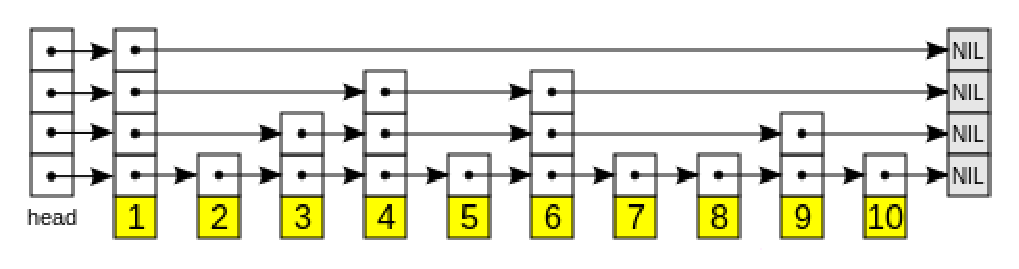
\includegraphics[scale=0.75]{skiplist.eps}
\caption{Estructura de Skip List.}
\label{fig:skip}
\end{figure}

La estructura de una Skip List se aprecia en la figura \ref{fig:skip}. La altura de cada nodo (cantidad de $duplicados$ que tiene en listas superiores) se determina del siguiente modo: se elige con probabilidad $\frac{1}{2}$ si el nodo tiene un duplicado en el nivel $i$ (comenzando con $i=2$), y en caso afirmativo se procede con la elección para el nivel $i+1$, en caso negativo se termina el proceso. Todo nodo tiene al menos altura $1$ (está presente en la primera lista).\\

Para implementar esta estructura se definieron las clases SkipNode y SkipList.

\subsubsection{Clase SkipNode}
Representa a cada nodo y sus duplicados en listas superiores. Consiste simplemente en una llave $key$ y una lista $next$ de tamaño $n$, donde para cada $i \in [0,n)$, $next_{i}$ es un puntero al siguiente elemento de la i-ésima lista de la Skip List.

\subsubsection{Clase SkipList}
Representa a la lista en sí, la cual está conformada por un SkipNode $head$ y las operaciones de inserción y búsqueda.\\

La inserción funciona del siguiente modo:

\begin{itemize}
\item	Se crea un SkipNode $node$ con la llave $k$ que se desea insertar, y una altura determinada con el método explicado en \ref{sec:sl}.
\item	Bla, bla, bla.
\end{itemize}


\subsection{ABB}
El ABB se implementó con una clase $Node$ y una clase $ABB$. Cada objeto $Node$ contiene una llave $key$ y los punteros a sus hijos $left$ y $right$. Una instancia de $ABB$ contiene a un objeto $Node$ $root$ y las operaciones $insert$ y $search$. Ambas operaciones consisten en una mera búsqueda binaria, que en el caso de la inserción al encontrar un nodo vacío ($None$) inserta un nuevo nodo en ese espacio. Las operaciones se implementaron de forma iterativa en  vez de recursiva para evitar el desbordamiento de la pila, ya que Python no provee optimización de llamada por la cola.

\subsection{ABB Aleatorizado}
Para el ABB Aleatorizado se creó la clase $ABBRandom$ que extiende de $ABB$. En este árbol cada vez que se agrega un nodo se debe determinar si éste se convertirá en la raíz, lo cual ocurre con probabilidad $\frac{1}{n}$. Para esto se obtiene un número pseudoaleatorio entre 1 y $n$ con distribución uniforme mediante la función $randint$ que provee el lenguaje, donde $n$ es la cantidad de nodos del árbol, y si este número es igual a $n$ entonces el nodo se convierte en raíz.\\

Para que un nodo se convierta en raíz manteniendo la consistencia del árbol lo que se hace es rotarlo desde su posición de inserción hasta que quede en la raíz del árbol. Para hacer esto se añadió el campo $parent$ (referencia al nodo padre) a la clase $Node$, para facilitar la implementación de las rotaciones.\\

Un nodo $node$ se lleva desde su posición de inserción a la raíz $root$ del árbol del siguiente modo:
\begin{itemize}
\item	Mientras $node.parent \not= None$:
	\begin{itemize}
	\item	Si $node.parent.left = node$, $node := rotateRight(node)$
	\item	En otro caso, $node := rotateLeft(node)$
	\end{itemize}
\item	$root := node$
\end{itemize}

\begin{figure}[ht]
\centering
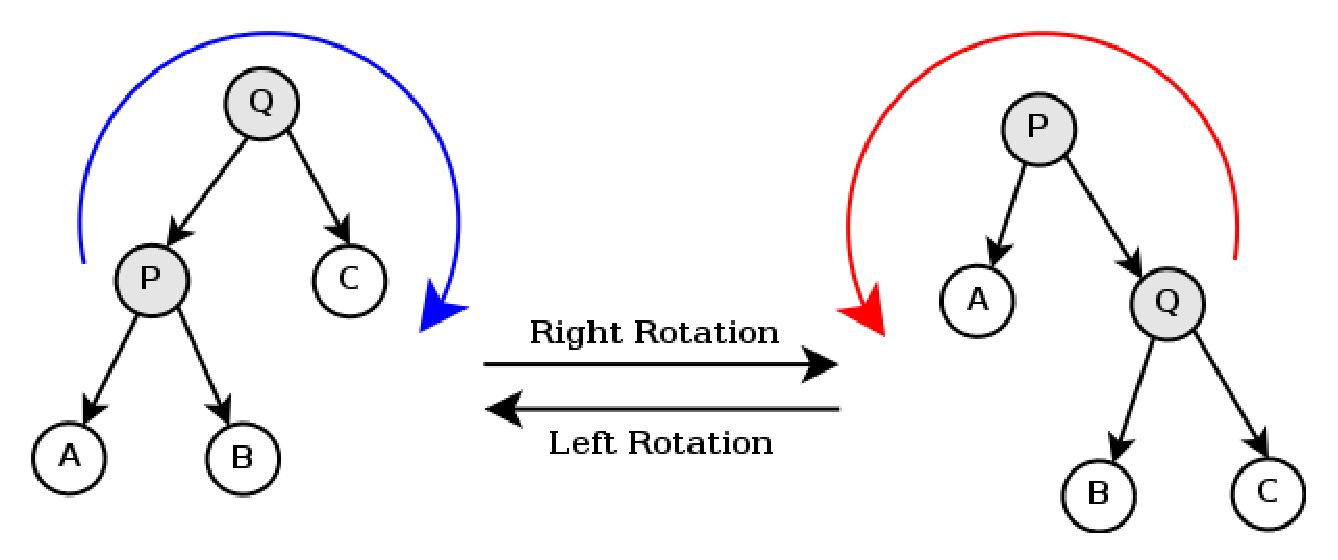
\includegraphics[scale=0.7]{rotations.eps}
\caption{Operaciones de rotación de nodos, hacia la derecha e izquierda.}
\label{fig:rotaciones}
\end{figure}

\section{Experimentos}


\section{Conclusión}


%\end{doublespace}
\end{document}